\section{Procedure}

So far, the problem has been introduced and the required terminology has been defined. Recall that there are two 
changes; the insertion/deletion of bars or relocation of bars.
However, there has yet to be discussion regarding the two 
listing algorithms. In the procedure section 
we look at each of the algorithms and explain what 
each of the algorithms are doing. The goal is to transition from 
$L_{i}$ to $L_{i+1}$ in $CanL{\pi_{N}}$ with minimal change, which means adding or removing 
the least number of bars to get from $L_{i}$ to $L_{i+1}$ or relocating 
the least number of bars to get from $L_{i}$ to $L_{i+1}$.\par 

The reason that the modified SJT and CI algorithms were chosen is because they allow 
for minimal change from $L_{i}$ to $L_{i+1}$. While conducting this research, modifications 
to the permutation listing algorithms mentioned in chapter one were applied for listing $CanL\{\pi_{N}\}$. Recall that 
these listing algorithms were Zaks, Heaps, and Lexicographic. These listing algorithms 
did not allow for minimal change when transitioning from $L_{i}$ to $L_{i+1}$.
%%section SJT
\subsection{Steinhaus-Johnson-Trotter}
\begin{algorithm}
  \caption{Modified SJT algorithm for processing at $K=N$}
  \begin{algorithmic}[1]
    \Function{modifiedSjt}{$N$, $Ladder[2(N-1)-1][N-1]$, $Arr[N-1]$, $Direction[N]$}


      \State $print(Ladder)$

      %%base case
      \If{$GlobalCount = N!$}
        \State return
      \EndIf

     
      %%swap the nth element n-1 times
      \For{$i \gets 1$,$i < N$, $i \gets i+1$}
        
        \If{$Direction[N] = left$}
            \State $row \gets (N) - i$
            \State $col \gets row$
            \State $Ladder[row][col] \gets 1$
        \Else
            \State $row \gets i$
            \State $col \gets row$
            \State $Ladder[row][col] \gets 0$
        \EndIf
        \State $GlobalCount \gets GlobalCount+1$
        \State $print(Ladder)$

      \EndFor
      \State $Direction[N] \gets !Direction[N]$
      \State $K \gets N-1$
      \State $HELPERSJT(K, N, Ladder, Arr, Direction)$
      \State $MODIFIEDSJT(N,  Ladder, Arr, Direction)$

    \EndFunction
  \end{algorithmic}
\end{algorithm}

%%helper algorithm
\begin{algorithm}
  \caption{Helper SJT algorithm for processing when $2 \leq K < N$}
  \begin{algorithmic}[1]
    \Function{helpersjt}{$N$, $K=(N-1)$, $Ladder[2(N-1)-1][N-1]$, $Arr[N-1]$, $Direction[N]$}

      \For{$i \gets K$, $i \geq 1$, $i \gets i-1$}
        \If{$Arr[K] < K$}
        \State $GlobalCount \gets GlobalCount + 1$

          \If{$Direction[K] = LEFT$}
            \State $row \gets (N-1) + (N-K) - arr[K]$
            \State $col \gets (K) - arr[K]$
            \State $Ladder[row][col] \gets 1$

          \Else
            \State $row \gets  (N-1) + (N-K) + arr[K] - (K-2)$
            \State $col \gets arr[K]$
            \State $Ladder[row][col] \gets 0$
          \EndIf
          \State $Arr[K]\gets arr[K]+1$
          \State return
        \Else 
          \State $Arr[K] \gets 0$
          \State $Direction[K] \gets !Direction[K]$
        \EndIf
        $K \gets K-1$
      \EndFor
      \EndFunction
  \end{algorithmic}
\end{algorithm}
\pagebreak

Let the \emph{identity ladder} be the ladder for the sorted permutation from $[1 \dots N]$.
Let the initial conditions of the algorithm be the fallowing. The $Ladder= 2D array$ initialized to the identity ladder,  
let $N \geq 1$, let $Arr$ be a one indexed array initialized to zero for all indexes. Let $Direction$ be a one 
indexed array set to false for all indexes. The principles of the algorithm are the following, if the direction for a 
given route is false, then bars will be added for that given route, from right to left, bottom to top, until no more bars can be added. Let a 
$1$ at $Ladder[row][col]$ indicate a bar has been added to the ladder at the given row and column.
If the direction for a given route is true, then bars will be removed for that given route, left to right, top to bottom, until 
no more bars can be removed. Let a $0$ at $Ladder[row][col]$ indicate a bar has been removed from the ladder 
at the given row and column. Let $K$ be the value of some given route where $1 < K < N$. Note that element one has no route.
The number of bars for a given route is $1 \leq K < N-1$. This is because the maximum number of inversions 
the $Kth$ element can make is $K-1$, therefore the $Kth$ route can have at most $N-2$, if $K=N-1$, and 
at least $1$ bar if $K=2$. Once all the bars for the $Kth$ route have been added 
or removed, the direction for the $Kth$ route is switched, indicating that its bars will be removed if they 
were added, or added if they were removed. Once all the bars for the $Kth$ route have been added or removed, 
the next bar of the $K-1th$ route will be added or removed. Once this is done, the bars of route $K$ will 
then be added if they were previously removed or removed if previously added. Repeat this process until all
$N!$ ladders have been generated.

\subsubsection{Proof} 
Since the alorithm is a modification of the Steinhaus-Johnson-Trotter algorithm, a similar proof for the SJT algorithm 
can be applied to the modified SJT algorithm for ladder-lotteries. Suppose we want to generate all ladders 
of order $N$ using the modified SJT algorithm. Suppose we had all ladders of order $N-1$, then for 
each ladder of order $N-1$, add a line to the ladder of order $N-1$ to get a ladder of order $N$. Call these ladders 
$L_{(N-1)+1}$. For each $L_{(N-1)+1}$, if it is an odd numbered ladder, then add a bar to each column from bottom right 
to top left. This can be done $(N-1)$ times resulting in $N$ ladders derived from the odd numbered 
$L_{(N-1)+1}$ ladder; the first ladder equals odd numbered $L_{(N-1)+1}$. 
If it is an even numbered ladder, then add $(N-1)$ bars from top left to bottom right to get the first ladder 
of order $N$ from the even numbered $L_{(N-1)+1}$. Then proceed to remove the $(N-1)$ bars from top left to bottom right. 
Removing $(N-1)$ bars results in $N$ ladders derived from the even numbered ladder $L_{(N-1)+1}$ ladder; the first ladder 
is $L_{(N-1)+1}$ with the $(N-1)$ ladders added to it from top left to bottom right. Also note that the last ladder derived from 
the odd $L_{(N-1)+1}$ is the same as the first ladder derived from the subsequent even numbered $L_{(N-1)+1}$ with the exception 
of an additional bar in the subsequent even $L_{(N-1)+1}$. Thus, the last ladder of order $N$ derived from 
the odd numbered $L_{(N-1)+1}$ requires one bar insertion to get to the first ladder of order $N$ derived from the subsequent 
even numbered $L_{(N-1)+1}$. Continue this process for all $L_{(N-1)+1}$ and string the results together, thus 
listing all ladders of order $N$. To see an example for $N=4$ please refer to figure \ref{Fig:CanLSJT}.\pagebreak

%%prove the dimensions of the datastructure
\begin{center}
\begin{figure}[!htp]

  %%First tree
  \begin{minipage}{.9\textwidth}
  
  \resizebox{.9\textwidth}{.45\textheight}{
  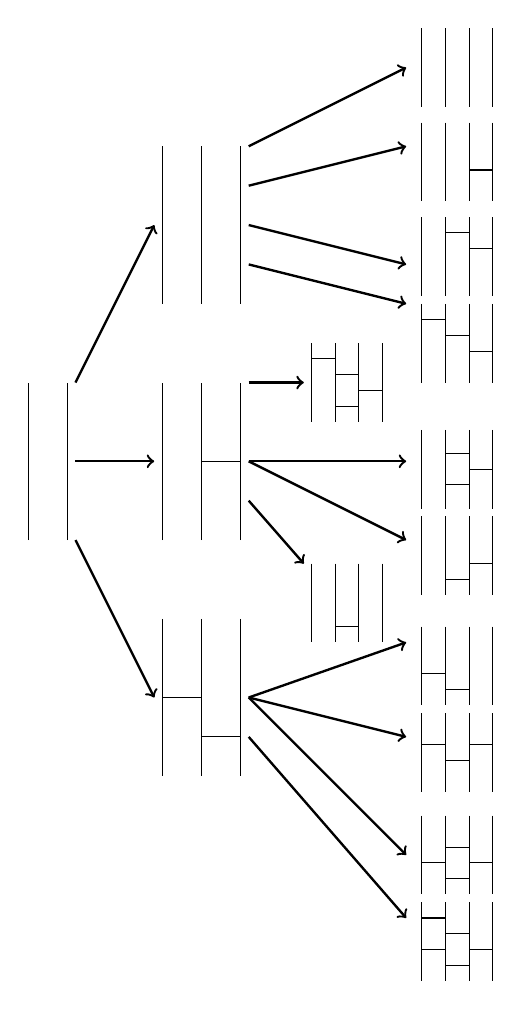
\begin{tikzpicture}
   
  %%t1
  \draw(0, 5) to (0, 7);
  \draw(.5, 5) to (.5, 7);

  \draw[->, line width = .3mm](.6, 7) to (1.6, 9);
  \draw[->, line width = .3mm](.6, 6) to (1.6, 6);
  \draw[->, line width = .3mm](.6, 5) to (1.6, 3);

    \draw(1.7, 10) to (1.7, 8);
    \draw(2.2, 10) to (2.2, 8);
    \draw(2.7, 10) to (2.7, 8);

      \draw[->, line width = .3mm](2.8, 10) to (4.8, 11);
      \draw[->, line width = .3mm](2.8, 9.5) to (4.8, 10);
      \draw[->, line width = .3mm](2.8, 9) to (4.8, 8.5);
      \draw[->, line width = .3mm](2.8, 8.5) to (4.8, 8);

        \draw(5, 10.5) to (5, 11.5);
        \draw(5.3, 10.5) to (5.3, 11.5);
        \draw(5.6, 10.5) to (5.6, 11.5);
        \draw(5.9, 10.5) to (5.9, 11.5);

        \draw(5, 10.3) to (5, 9.3);
        \draw(5.3, 10.3) to (5.3, 9.3);
        \draw(5.6, 10.3) to (5.6, 9.3);
          \draw(5.6, 9.7) to (5.9, 9.7);
        \draw(5.9, 10.3) to (5.9, 9.3);

        \draw(5, 9.1) to (5, 8.1);
        \draw(5.3, 9.1) to (5.3, 8.1);
          \draw(5.3, 8.9) to (5.6, 8.9);
        \draw(5.6, 9.1) to (5.6, 8.1);
          \draw(5.6, 8.7) to (5.9, 8.7);
        \draw(5.9, 9.1) to (5.9, 8.1);

        \draw(5, 8) to (5, 7);
          \draw(5, 7.8) to (5.3, 7.8);
        \draw(5.3, 8) to (5.3, 7);
          \draw(5.3, 7.6) to (5.6, 7.6);
        \draw(5.6, 8) to (5.6, 7);
          \draw(5.6, 7.4) to (5.9, 7.4);
        \draw(5.9, 8) to (5.9, 7);
  %%t2
  \draw(1.7, 5) to (1.7, 7);
  \draw(2.2, 5) to (2.2, 7);
    \draw(2.2, 6) to (2.7, 6);
  \draw(2.7, 5) to (2.7, 7);
    
    \draw[->, line width = .3mm](2.8, 7) to (3.5, 7);
    \draw[->, line width = .3mm](2.8, 6) to (4.8, 6);
    \draw[->, line width = .3mm](2.8, 6) to (4.8, 5);
    \draw[->, line width = .3mm](2.8, 5.5) to (3.5, 4.7);

      \draw(3.6, 7.5) to (3.6, 6.5);
        \draw(3.6, 7.3) to (3.9, 7.3);
      \draw(3.9, 7.5) to (3.9, 6.5);
        \draw(3.9, 6.7) to (4.2, 6.7);
        \draw(3.9, 7.1) to (4.2, 7.1); 
      \draw(4.2, 7.5) to (4.2, 6.5);
        \draw(4.2, 6.9) to (4.5, 6.9);
      \draw(4.5, 7.5) to (4.5, 6.5);

      
      \draw(5, 6.4) to (5, 5.4);
      \draw(5.3, 6.4) to (5.3, 5.4);
        \draw(5.3, 6.1) to (5.6, 6.1);
        \draw(5.3, 5.7) to (5.6, 5.7);
      \draw(5.6, 6.4) to (5.6, 5.4);
        \draw(5.6, 5.9) to (5.9, 5.9);
      \draw(5.9, 6.4) to (5.9, 5.4);

  
      \draw(5, 5.3) to (5, 4.3);
      \draw(5.3, 5.3) to (5.3, 4.3);
        \draw(5.3, 4.5) to (5.6, 4.5);
      \draw(5.6, 5.3) to (5.6, 4.3);
        \draw(5.6, 4.7) to (5.9, 4.7);
      \draw(5.9, 5.3) to (5.9, 4.3);

  
      \draw(3.6, 4.7) to (3.6, 3.7);
      \draw(3.9, 4.7) to (3.9, 3.7);
        \draw(3.9, 3.9) to (4.2, 3.9);
      \draw(4.2, 4.7) to (4.2, 3.7);
      \draw(4.5, 4.7) to (4.5, 3.7);

  %%t3

 
  
  \draw(1.7, 4) to (1.7, 2);
    \draw(1.7, 3) to (2.2, 3);
  \draw(2.2, 4) to (2.2, 2);
    \draw(2.2, 2.5) to (2.7, 2.5);
  \draw(2.7, 4) to (2.7, 2);
    
    \draw[->, line width = .3mm](2.8, 3) to (4.8, 3.7);
    \draw[->, line width = .3mm](2.8, 3) to (4.8, 2.5);
    \draw[->, line width = .3mm](2.8, 3) to (4.8, 1);
    \draw[->, line width = .3mm](2.8, 2.5) to (4.8, .2);

  \draw(5, 3.9) to (5, 2.9);
    \draw(5, 3.3) to (5.3, 3.3);
  \draw(5.3, 3.9) to (5.3, 2.9);
    \draw(5.3, 3.1) to (5.6, 3.1);
  \draw(5.6, 3.9) to (5.6,2.9);
  \draw(5.9, 3.9) to (5.9, 2.9);
    

  \draw(5, 2.8) to (5, 1.8);
    \draw(5, 2.4) to (5.3, 2.4);
  \draw(5.3, 2.8) to (5.3, 1.8);
    \draw(5.3, 2.2) to (5.6, 2.2);
  \draw(5.6, 2.8) to (5.6,1.8);
    \draw(5.6, 2.4) to (5.9, 2.4);
  \draw(5.9, 2.8) to (5.9, 1.8);
  

  \draw(5, 1.5) to (5, .5);
    \draw(5, .9) to (5.3, .9);
  \draw(5.3, 1.5) to (5.3, .5);
    \draw(5.3, .7) to (5.6, .7);
    \draw(5.3, 1.1) to (5.6, 1.1);
  \draw(5.6, 1.5) to (5.6,.5);
    \draw(5.6, .9) to (5.9, .9);
  \draw(5.9, 1.5) to (5.9, .5);
  

  \draw(5, .4) to (5, -.6);
    \draw(5, .2) to (5.3, .2);
    \draw(5, -.2) to (5.3, -.2);
  \draw(5.3, .4) to (5.3, -.6);
    \draw(5.3, 0) to (5.6, 0);
    \draw(5.3, -.4) to (5.6, -.4);
  \draw(5.6, .4) to (5.6,-.6);
    \draw(5.6, -.2) to (5.9, -.2);
  \draw(5.9, .4) to (5.9, -.6);



  \end{tikzpicture}}
  \end{minipage}

   %%Second tree
  \begin{minipage}{.9\textwidth}
  
  
  \resizebox{.9\textwidth}{.45\textheight}{
  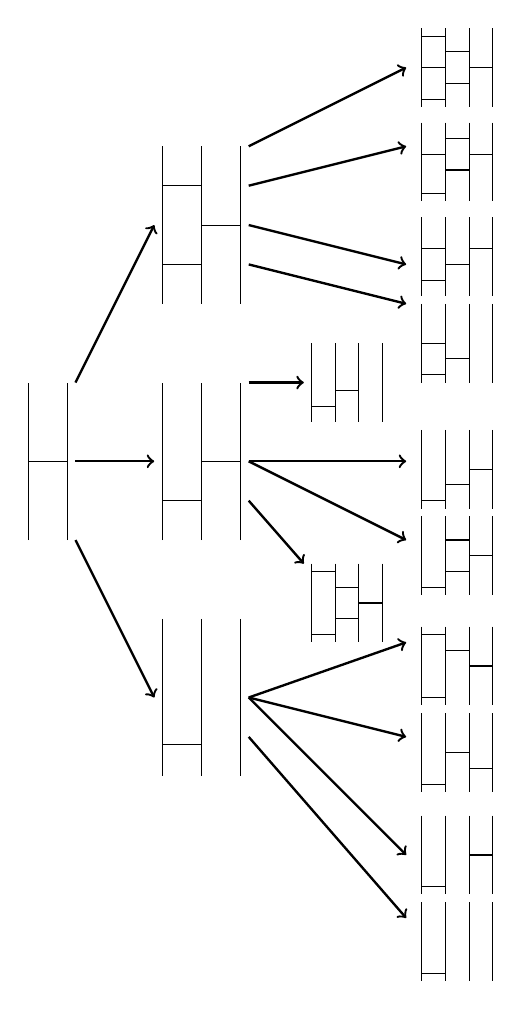
\begin{tikzpicture}
   
  %%t1
  \draw(0, 5) to (0, 7);
    \draw(0, 6) to (.5, 6);
  \draw(.5, 5) to (.5, 7);

  \draw[->, line width = .3mm](.6, 7) to (1.6, 9);
  \draw[->, line width = .3mm](.6, 6) to (1.6, 6);
  \draw[->, line width = .3mm](.6, 5) to (1.6, 3);

    \draw(1.7, 10) to (1.7, 8);
      \draw(1.7, 9.5) to (2.2, 9.5);
      \draw(1.7, 8.5) to (2.2, 8.5);
    \draw(2.2, 10) to (2.2, 8);
      \draw(2.2, 9) to (2.7, 9);
    \draw(2.7, 10) to (2.7, 8);

      \draw[->, line width = .3mm](2.8, 10) to (4.8, 11);
      \draw[->, line width = .3mm](2.8, 9.5) to (4.8, 10);
      \draw[->, line width = .3mm](2.8, 9) to (4.8, 8.5);
      \draw[->, line width = .3mm](2.8, 8.5) to (4.8, 8);

        \draw(5, 10.5) to (5, 11.5);
          \draw(5, 11.4) to (5.3, 11.4);
          \draw(5, 11) to (5.3, 11);
          \draw(5, 10.6) to (5.3, 10.6);
        \draw(5.3, 10.5) to (5.3, 11.5);
          \draw(5.3, 11.2) to (5.6, 11.2);
          \draw(5.3, 10.8) to (5.6, 10.8);
        \draw(5.6, 10.5) to (5.6, 11.5);
          \draw(5.6, 11) to (5.9, 11);
        \draw(5.9, 10.5) to (5.9, 11.5);

        \draw(5, 10.3) to (5, 9.3);
          \draw(5, 9.9) to (5.3, 9.9);
          \draw(5, 9.4) to (5.3, 9.4);
        \draw(5.3, 10.3) to (5.3, 9.3);
          \draw(5.3, 10.1) to (5.6, 10.1);
          \draw(5.3, 9.7) to (5.6, 9.7);
        \draw(5.6, 10.3) to (5.6, 9.3);
          \draw(5.6,  9.9) to (5.9, 9.9);
        \draw(5.9, 10.3) to (5.9, 9.3);

        \draw(5, 9.1) to (5, 8.1);
          \draw(5, 8.7) to (5.3, 8.7);
          \draw(5, 8.3) to (5.3, 8.3);
        \draw(5.3, 9.1) to (5.3, 8.1);
          \draw(5.3, 8.5) to (5.6, 8.5);
        \draw(5.6, 9.1) to (5.6, 8.1);
          \draw(5.6, 8.7) to (5.9, 8.7);
        \draw(5.9, 9.1) to (5.9, 8.1);

        \draw(5, 8) to (5, 7);
          \draw(5, 7.5) to (5.3, 7.5);
          \draw(5, 7.1) to (5.3, 7.1);
        \draw(5.3, 8) to (5.3, 7);
          \draw(5.3, 7.3) to (5.6, 7.3);
        \draw(5.6, 8) to (5.6, 7);
        \draw(5.9, 8) to (5.9, 7);
  %%t2
  \draw(1.7, 5) to (1.7, 7);
    \draw(1.7, 5.5) to (2.2, 5.5);
  \draw(2.2, 5) to (2.2, 7);
    \draw(2.2, 6) to (2.7, 6);
  \draw(2.7, 5) to (2.7, 7);
    
    \draw[->, line width = .3mm](2.8, 7) to (3.5, 7);
    \draw[->, line width = .3mm](2.8, 6) to (4.8, 6);
    \draw[->, line width = .3mm](2.8, 6) to (4.8, 5);
    \draw[->, line width = .3mm](2.8, 5.5) to (3.5, 4.7);

      \draw(3.6, 7.5) to (3.6, 6.5);
        \draw(3.6, 6.7) to (3.9, 6.7);
      \draw(3.9, 7.5) to (3.9, 6.5);
        \draw(3.9, 6.9) to (4.2, 6.9);
      \draw(4.2, 7.5) to (4.2, 6.5);
      \draw(4.5, 7.5) to (4.5, 6.5);

      
      \draw(5, 6.4) to (5, 5.4);
        \draw(5, 5.5) to (5.3, 5.5);
      \draw(5.3, 6.4) to (5.3, 5.4);
        \draw(5.3, 5.7) to (5.6, 5.7);
      \draw(5.6, 6.4) to (5.6, 5.4);
        \draw(5.6, 5.9) to (5.9, 5.9);
      \draw(5.9, 6.4) to (5.9, 5.4);

  
      \draw(5, 5.3) to (5, 4.3);
        \draw(5, 4.4) to (5.3, 4.4);
      \draw(5.3, 5.3) to (5.3, 4.3);
        \draw(5.3, 4.6) to (5.6, 4.6);
        \draw(5.3, 5) to (5.6, 5);
      \draw(5.6, 5.3) to (5.6, 4.3);
        \draw(5.6, 4.8) to (5.9, 4.8); 
      \draw(5.9, 5.3) to (5.9, 4.3);

  
      \draw(3.6, 4.7) to (3.6, 3.7);
        \draw(3.6, 4.6) to (3.9, 4.6);
        \draw(3.6, 3.8) to (3.9, 3.8);
      \draw(3.9, 4.7) to (3.9, 3.7);
        \draw(3.9, 4.4) to (4.2, 4.4);
        \draw(3.9, 4) to (4.2, 4);
      \draw(4.2, 4.7) to (4.2, 3.7);
        \draw(4.2, 4.2) to (4.5, 4.2);
      \draw(4.5, 4.7) to (4.5, 3.7);

  %%t3



  \draw(1.7, 4) to (1.7, 2);
    \draw(1.7, 2.4) to (2.2, 2.4);
  \draw(2.2, 4) to (2.2, 2);
  \draw(2.7, 4) to (2.7, 2);
    
    \draw[->, line width = .3mm](2.8, 3) to (4.8, 3.7);
    \draw[->, line width = .3mm](2.8, 3) to (4.8, 2.5);
    \draw[->, line width = .3mm](2.8, 3) to (4.8, 1);
    \draw[->, line width = .3mm](2.8, 2.5) to (4.8, .2);

  \draw(5, 3.9) to (5, 2.9);
    \draw(5, 3) to (5.3, 3);
    \draw(5, 3.8) to (5.3, 3.8);
  \draw(5.3, 3.9) to (5.3, 2.9);
    \draw(5.3, 3.6) to (5.6, 3.6);
  \draw(5.6, 3.9) to (5.6,2.9);
    \draw(5.6, 3.4) to (5.9, 3.4);
  \draw(5.9, 3.9) to (5.9, 2.9);
    

  \draw(5, 2.8) to (5, 1.8);
    \draw(5, 1.9) to (5.3, 1.9);
  \draw(5.3, 2.8) to (5.3, 1.8);
    \draw(5.3, 2.3) to (5.6, 2.3);
  \draw(5.6, 2.8) to (5.6,1.8);
        \draw(5.6, 2.1) to (5.9, 2.1);
  \draw(5.9, 2.8) to (5.9, 1.8);
  

  \draw(5, 1.5) to (5, .5);
    \draw(5, .6) to (5.3, .6);
  \draw(5.3, 1.5) to (5.3, .5);
  \draw(5.6, 1.5) to (5.6, .5);
    \draw(5.6, 1) to (5.9, 1);
  \draw(5.9, 1.5) to (5.9, .5);
  

  \draw(5, .4) to (5, -.6);
    \draw(5, -.5) to (5.3, -.5);
  \draw(5.3, .4) to (5.3, -.6);
  \draw(5.6, .4) to (5.6,-.6);
  \draw(5.9, .4) to (5.9, -.6);
  



  \end{tikzpicture}}
  \end{minipage}




  \caption{$CanL\{\pi_{4}\}$ generated by the modified SJT algorithm. The algorithm inserts or removes a bar from the previous 
  ladder at the leaf nodes in the tree, the tree is used to prove the veracity of the algorithm}
  \label{Fig:CanLSJT}
\end{figure}
\end{center}




\begin{theorem}
  The number of rows required for the ladder data-structure is $2(N-1) - 1$ and the number of columns required for 
  the ladder is $N-1$.
\end{theorem}
\begin{proof}
  The number of columns is fairly straighforward. Seeing as there are always $N$ elements in $\pi_{N}$, 
  a column represents a gap between lines in the corresponding ladder-lottery. Each ladder of order $N$ has $N$ lines, 
  one for each element in $\pi_{N}$. Therefore each ladder of order $N$ has $N-1$ columns.\par 
  The number of rows for the ladder data-structure is calculated a follows, given $\pi_{N}$, the minimal 
  number of rows required is when $\pi_{N}$ is sorted. In this case there are zero rows because there are 
  zero bars added to the ladder. This ladder is $L_{N_{ID}}$ and is 
  the first ancestor in $CanL\{\pi_{N}\}$. When a bar is added to the ladder it can be added to an already existing row 
  or to a new row. If the current state of the ladder is $L_{N_{ID}}$ then adding the first bar creates the second ladder in
  $CanL\{\pi_{N}\}$. Since the bars are being added bottom right to top left, and the first bar to be added belongs 
  to the $Nth$ route, then it must be added to $row=N-1$, $col=N-1$. As bars of the $Nth$ route get 
  continuously added to the ladder, each bar is added a row above the previous bar and to a column 
  to the left of the column of the previous bar.
  Since no two bars of the $Nth$ route can be on the same row, this will require $N-1$ rows. Note, if they were added to the same 
  row, then the left end point of the right bar would be touching the right end point of the left bar which is disallowed. Once the 
  bars of the $Nth$ element are added, the bars of the $N-1th$ route will be added. The $N-1th's$ first bar 
  will be added to the $N-2$ column, otherwise it would be directly below the first bar of the $Nth$ route, which is a violation. 
  Since the first bar of the $N-1$'s element is added to column $N-2$, then it must be given a new row, otherwise its right end point 
  will be touching  the left end point of the first bar of route $N$. The remaining $N-2$ bars of element $N-1$
  will be added bottom right to top left, but none of their end points will touch the end points of element $N$ seeing as they will 
  always be two columns apart from any bar in $N's$ route. The same logic applies to element $N-2$, it will require one extra row for its 
  first bar, in order not to touch the first bar of element $N-1$, but the remainder of its bars will always be two columns away from 
  the remainder of the bars for $N-1$, etc. Therefore there are $N-1$ rows required for the $Nth$ element and each subsequent 
  element, $K$ requires only one new row. Since $2 \leq K < N$, then there are $(N-2)$ additional rows required for the ladder. Note that element 
  $1$ has no bars in its route. Therefore there are $(N-1)$ rows required for element $N's$ bars  plus $(N-2)$ rows required for 
  all the remaining $2 \leq K < N$ routes. In conclusion the number of rows required is $(N-1) + (N-2) = 2(N-1)-1$. See figure for the tree of ladders 
  generated by modified SJT for $N=4$. Note that the maximum number of rows required is $2(N-1)-1=2(3)-1=5$.
\end{proof}



%%end proof


From Fig. \ref{Fig:CanLSJT} it should be clear that the canonical representative from $CanL{\pi_{N}}$ when using the 
Modified SJT algorithm is also the root ladder from each $OptL{\pi_{N}}$. Recall that the root ladder is the 
ladder whose bars of a lesser route have not crossed the bars of a greater route. In the case of the 
Modified SJT algorithm, transitioning from $L_{i}$ to $L_{i+1}$ involves simply inserting a new bar 
or removing a bar for a given route. Let $K$ be the current route. If a new bar being added belongs to 
route $K$, then the addition of the bar does not violate the property of the root ladder. If the new bar to
be added belongs to route $K-1$, then the bar is added below $K's$ bars, still not violating the property of 
the root ladder. When a bar is removed, that implies it has already been added. Let $L_{i}$ be a 
ladder whose bar is about to be removed, thus transitioning to $L_{i+1}$. Let $L_{i}$ be a root ladder
, then removing a bar from $L_{i}$ cannot make $L_{i+1}$ a non-root ladder, because 
removing a bar from $L_{i}$ does not allow the bar of a lesser element to cross the bars of a greater element.
Thus, the canonical representative for $CanL{\pi_{N}}$ is always the root ladder from each $OptL{\pi_{N}}$.\par 



%%Beging the cases
The calculations for the row and column for the bar 
depend on several factors. The first factor is whether the row and column is being calculated for $route=N$ or 
if $route < N$. If $route=N$, then the row and column are calculated using the main function, ModifiedSJT. The second factor 
is whether a bar is being removed from the ladder or a bar is being added to the ladder. Therefore, there are eight cases 
to consider. The cases are the following: 
\begin{caseof}
  \case{$Route = N$}{Bar is being added. Row is being calculated.}
  \case{$Route = N$}{Bar is being added. Column is being calculated.}
  \case{$Route = N$}{Bar is being removed. Row is being calculated.}
  \case{$Route = N$}{Bar is being removed. Column is being calculated.}
  \case{$Route < N$}{Bar is being added. Row is being calculated.}
  \case{$Route < N$}{Bar is being added. Column is being calculated.}
  \case{$Route < N$}{Bar is being removed. Row is being calculated.}
  \case{$Route < N$}{Bar is being removed. Column is being calculated.}
\end{caseof}

%%End the cases

When proving the above cases, keep in mind that the ladder, $L$, is a two dimensional array with $2(N-1)-1$ rows and $(N-1)$ columns.

%%proof 1
\begin{lemma}
  Let $route=N$. Let $I=$ the current number of bars in the ladder belonging to route $N$. 
  Assume a bar is being added. Then the $row=(N-1)-I$.
\end{lemma}
\begin{proof}
  Keeping in mind we are only dealing with root ladders, then the bars of the $Nth$ route will be above the bars of 
  any other route. The bars are added bottom right to top left, and no two bars of the $Nth$ route can be on the same row.
  There are a total of $N-1$ rows requried for the bars of the $Nth$ route. $I$ is incremented for each bar that is added 
  to the $Nth$ route. The first bar to be added will be at row $N-1$, once it is added $I$ is incremented by one, the second 
  bar of the $Nth$ route will be added to row $N-2$, which equals $N-1-I$. Then $I$ is incremented again. This continues 
  until all bars of the $Nth$ route are added. Refer to Fig. \ref{fig:SJTcase1} for an example of row calulation when adding a bar 
  for the $Nth$ route.
\end{proof}
\begin{figure}[!htp]
  \begin{center}
    \begin{tikzpicture}
      \draw(0, 0) to (0, 6);
      \draw(2, 0) to (2, 6);
        \node at(3, 4.7){4,2};
        \draw(2, 4.5) to (4, 4.5);
      \draw(4, 0) to (4, 6);
        \node at(5, 3.7){4,3};
        \draw(4, 3.5) to (6, 3.5);
      \draw(6, 0) to (6, 6);

      \node at(-2, 5.5){R1};
      \node at(-2, 4.5){R2};
      \node at(-2, 3.5){R3};
      \node at(-2, 2.5){R4};
      \node at(-2, 1.5){R5};

      \node at(0, 6.2){1};
      \node at(2, 6.2){4};
      \node at(4, 6.2){2};
      \node at(6, 6.2){3};

      \draw (1,5.5) ellipse (1cm and .4cm);

    \end{tikzpicture}
  \end{center}
  \caption{The row of the last bar to be added for element $4$ is row $1$. $row=1=3-2=(N-1)-I$}
  \label{fig:SJTcase1}
\end{figure}

%%end proof 1


%%Prove case 2
\begin{lemma}
  Let $route=N$. Let $I=$ the current number of bars in the ladder belonging to route $N$. 
  Assume a bar is being added. Then the $column=(N-1)-I$.
\end{lemma}
\begin{proof}
  Keeping in mind we are only dealing with root ladders, then the bars of the $Nth$ route will be above the bars of 
  any other route. The bars are added bottom right to top left. The ladder has a total of $N-1$ columns, seeing as 
  the $Nth$ element has $N-1$ bars, each requiring their own column. If two bars of the $Nth$ element were 
  in the same column, then this would violate one of two constraints. Either the two bars would be directly 
  above/below each other, in which case the ladder would not be optimal seeing as the two elements that crossed the 
  top bar would then cross the bottom bar, which means the ladder has an extra bar. The second case can be discredited as 
  follows. Let the top bar belonging to route $N$ be designated as $X$, let the bottom bar belonging to route $N$ be 
  designated as $Y$. Assume $X$ and $Y$ are in the same column.
  Then there is some third bar $Z$, not belonging to route $N$ and not in the same column 
  as $X$ and $Y$ such that $Z$ is in the column directly to the left or right of the column of $X$ and $Y$. But if that 
  is the case, then $Z$ is above bar $Y$ which violates the definition of the root ladder. Therefore, every bar 
  belonging to route $N$ requires its own column. The first bar to be added to route $N$ goes in the rightmost column which 
  equals column $N-1$, then $I$ is incremented by one. The second bar is in column $(N-1)-1=(N-1)-I$ and $I$ is incremented 
  by one. The process continues until all $(N-1)$ bars of the $Nth$ route have been added. See figure \ref{fig:SJTcase2}for an example 
  of column calculation.
\end{proof}

\begin{figure}[!htp]
  \begin{center}
    \begin{tikzpicture}
       \draw(0, 0) to (0, 6);
      \draw(2, 0) to (2, 6);
        \node at(3, 4.7){4,2};
        \draw(2, 4.5) to (4, 4.5);
      \draw(4, 0) to (4, 6);
        \node at(5, 3.7){4,3};
        \draw(4, 3.5) to (6, 3.5);
      \draw(6, 0) to (6, 6);

      \node at(1, -0.3){Col 1};
      \node at(3, -0.3){Col 2};
      \node at(5, -0.3){Col 3};

      \node at(0, 6.2){1};
      \node at(2, 6.2){4};
      \node at(4, 6.2){2};
      \node at(6, 6.2){3};

      \draw (1,5.5) ellipse (1cm and .4cm);


      
    \end{tikzpicture}
  \end{center}
  \caption{The column of the last bar to be added for element $4$ is $1$. $column=1=3-2=(N-1)-I$}
  \label{fig:SJTcase2}
\end{figure}
%%End proof of case 2


%%Proof of case 3
\begin{lemma}
  Let $route=N$. Let $I=$ the current number of bars that have been removed from route $N$. Assume a bar is being removed. 
  Then the $row=I+1$
\end{lemma}
\begin{proof}
  Keeping in mind we are dealing with root ladders and bars are removed from left to right, top to bottom, then the first bar to 
  be removed from route $N$ is at row one. Since no bars have been removed, $I$ currently equals zero, 
  thus row $1=I+1$. Once removed, $I$ is increased by one, indicating a bar has been removed. The next bar is at row two, 
  which again equals $I+1$. Continue until all bars of the $Nth$ route have been removed. See figure \ref{fig:SJTcase3} for an example 
  of row calculation when removing a bar for the $Nth$ element.
\end{proof}
\begin{figure}[!htp]
  \begin{center}
    \begin{tikzpicture}
      \draw(0, 0) to (0, 6);
        \draw [dashed] (0,5.5) -- (2,5.5);
      \draw(2, 0) to (2, 6);
        \node at(3, 4.7){4,2};
        \draw(2, 4.5) to (4, 4.5);
      \draw(4, 0) to (4, 6);
        \node at(5, 3.7){4,3};
        \draw(4, 3.5) to (6, 3.5);
      \draw(6, 0) to (6, 6);

      \node at(-2, 5.5){R1};
      \node at(-2, 4.5){R2};
      \node at(-2, 3.5){R3};
      \node at(-2, 2.5){R4};
      \node at(-2, 1.5){R5};

      \node at(0, 6.2){1};
      \node at(2, 6.2){4};
      \node at(4, 6.2){2};
      \node at(6, 6.2){3};

      \draw (3,4.5) ellipse (1cm and .4cm);

    \end{tikzpicture}
  \end{center}
  \caption{The row of the second bar to be removed from element $4's$ route is row $2$. The dashed bar indicates that it has already been 
  removed from $4's$ route. $I$ is the number of bars currently removed from $4's$ route, which is currently $1$. Therefore $row=2=I+1$}
  \label{fig:SJTcase3}
\end{figure}

%%End of proof of case 3


%%Proof Case 4
\begin{lemma}
  Let $route=N$. Let $I=$ the current number of bars that have been removed from route $N$. Assume a bar is being removed.
  Then the $column=I+1$.
\end{lemma}
\begin{proof}
  Keeping in mind we are dealing with root ladders and bars are removed from left to right, top to bottom, then the first bar to 
  be removed from route $N$ is at column one. Since no bars have been removed, $I$ currently equals zero, 
  thus column $1=I+1$. Once removed, $I$ is increased by one, indicating a bar has been removed. The next bar is at column two, 
  which again equals $I+1$. Continue until all bars of the $Nth$ route have been removed. See figure \ref{fig:SJTcase4} for an example 
  of column calculation when removing a bar from the $Nth$ route.
\end{proof}

\begin{figure}[!htp]
  \begin{center}
    \begin{tikzpicture}
      \draw(0, 0) to (0, 6);
        \draw [dashed] (0,5.5) -- (2,5.5);

      \draw(2, 0) to (2, 6);
        \node at(3, 4.7){4,2};
        \draw(2, 4.5) to (4, 4.5);
      \draw(4, 0) to (4, 6);
        \node at(5, 3.7){4,3};
        \draw(4, 3.5) to (6, 3.5);
      \draw(6, 0) to (6, 6);

      \node at(1, -0.3){Col 1};
      \node at(3, -0.3){Col 2};
      \node at(5, -0.3){Col 3};

      \node at(0, 6.2){1};
      \node at(2, 6.2){4};
      \node at(4, 6.2){2};
      \node at(6, 6.2){3};

      \draw (3,4.5) ellipse (1cm and .4cm);


      
    \end{tikzpicture}
  \end{center}
  \caption{The column of the second bar to be removed from element $4's$ route is row $2$. The dashed bar indicates that it has already been 
  removed from $4's$ route. $I$ is the number of bars currently removed from $4's$ route, which currently is $1$. Therefore $column=2=I+1$}

  \label{fig:SJTcase4}
\end{figure}
%%End of proof of case 4



%%Proof of case 5
\begin{lemma}
  Let $Arr$ be a one indexed array. Let $K=route < N$. Let $2 \leq K < N$ be the $Kth$ element to have a bar added to its route. 
  Let $Arr[K]$ represent the number of bars for route $K$ that are currently in the 
  ladder. Let $L_{i}$ be a two dimensional, one indexed array representing the current ladder.
  The the row for the current bar to be added for route $K$ is $row=(N-1) + (N-K) - arr[K]$.
\end{lemma}
\begin{proof}
   It must be noted that we are listing only root ladders. So when transitioning from 
$L_{i}$ to $L_{i+1}$ in $CanL{\pi_{N}}$ both are root ladders. Recall that the root ladder is the ladder such that no  
route of any lesser value in $\pi$ has crossed the route of a greater value. With this in mind, one can say that the 
number of rows required for the $Nth$ value is $N-1$ seeing as the $Nth$ value can have at most $N-1$ bars in its route, each requiring  their own 
row. Since bars are added right to left, bottom, up, then the first bar of route $K$ will be added to the row 
just  below the last bar of the previous route. The reason $N-1$ is added is because the $Nth$ element requires 
$N-1$ rows in $L$. If $K$ is one less than $N$ then 
the first bar of $K$ will be added one row below the last bar of $N$. If $K$ is two less than $N$ then the first bar 
of $K$ will be added two rows below the last bar of $N$, etc. The $(N-K)$ is added because 
the difference between $N$ and $K$ is the offset of the difference in rows between the lowest/first bar of $N$ 
and the lowest/first bar of $K$. When a bar is added to $K's$ route, the $Arr[K]$ is incremented by one. This value is subtracted in 
order to effectively move up the ladder as bars are added to $K's$ route from bottom right to top left. See figure \ref{Fig:SJTcase5}for an example of 
row calculation when adding a bar for $K < N$.
\end{proof}\pagebreak

\begin{figure}[!htp]
  \begin{center}
    
    \begin{tikzpicture}

    \draw(0, -2) to (0, 6);
       \draw(0, 5.5) to (2, 5.5);
       \node at (1, 5.7){5,1};
       \node at (-1, 5.5){R1};
     \draw(2, -2) to (2, 6);
       \draw(2, 4.5) to (4, 4.5);
       \draw(2, 0.5) to (4, 0.5);
       \node at (3, 4.7){5,3};
       \node at(3, 0.7){3, 2};
       \node at(-1, 4.5){R2};
     \draw(4, -2) to (4, 6);
       \draw(4, 3.5) to (6, 3.5);
       \node at(5, 3.7){5,2};
       \node at(-1, 3.5){R3};
     \draw(6, -2) to (6, 6);
       \draw(6, 2.5) to (8, 2.5);
       \node at(7, 2.7){5,4};
       \node at(-1, 2.5){R4};
     \draw(8, -2) to (8, 6);

    \node at(-1, 1.5){R5};
    \node at(-1, 0.5){R6};
    \node at(-1, -0.5){R7};
    \draw (1,1.5) ellipse (1cm and .4cm);

  \end{tikzpicture}

\end{center}
\caption{The second bar of route 3 goes will go in row 5, column 1. $5 = (5-1)+(5-3)-1 = (N-1)+(N-K)-arr[K]$.}
\label{Fig:SJTcase5}
\end{figure}
%%End of prof of case 5


%%Proof of case 6
\begin{lemma}
  Let $Arr$ be a one indexed array. Let $route=K<N$. Let $2 \leq K < N$ be the $Kth$ element to have a bar added to its route. 
  Let $Arr[K]$ represent the number of bars for route $K$ that are currently in $L$. 
  The the column for the current bar to be added for route $K$ is $column=(K-1)-Arr[K]$.
\end{lemma}
\begin{proof}
  The total number of bars required for route $K$ is $K-1$, each requring their own column. The reason each 
  bar requires its own column is the same for when the route equals $N$. See the proof for lemma 3.1.5. The 
  bars are added right to left and when a bar is added $Arr[K]$ is incremented by one. The initial column to add the first bar 
  of route $K$ is column $K-1$. This is because the first bar of the $Kth$ route is the left child bar of the 
  lowest bar of the $K+1th$ route. Denote the first bar to be added of the $Kth$ route as $Y$ and the 
  lowest bar of the $K+1th$ route as $X$. $X$ is the parent bar of $Y$ and $Y$ is the left child bar of 
  $X$ for the following reasosn. If $Y$ was directly below $X$, then the ladder would have redundant bars, thus making it 
  non-optimal. If $Y$ was to the right of $X$, then $Y$ would either be above $X$, thus violating the property of the root ladder, 
  or if $Y$ were below $X$ and to the right of $X$ then $Y$ would be part of the route for $K+1$, yet this is a contradiction 
  seeing as we said $Y$ belongs to $K's$ route. Therefore, $Y$ must be in a column to the left of $X$. As bars are added 
  to $K's$ route, $Arr[K]$ is incremented for each bar. It is subtracted from the original column, $K-1$, effectively moving 
  to the next column to the left in $L$. See figure \ref{Fig:SJTcase6} for an example of column calculation when adding a bar for $K<N$.
\end{proof}
\begin{figure}[!htp]
  \begin{center}
    
    \begin{tikzpicture}

    \draw(0, -2) to (0, 6);
       \draw(0, 5.5) to (2, 5.5);
       \node at (1, 5.7){5,1};
     \draw(2, -2) to (2, 6);
       \draw(2, 4.5) to (4, 4.5);
       \draw(2, 0.5) to (4, 0.5);
       \node at (3, 4.7){5,3};
       \node at(3, 0.7){3, 2};
     \draw(4, -2) to (4, 6);
       \draw(4, 3.5) to (6, 3.5);
       \node at(5, 3.7){5,2};
     \draw(6, -2) to (6, 6);
       \draw(6, 2.5) to (8, 2.5);
       \node at(7, 2.7){5,4};
     \draw(8, -2) to (8, 6);

    \draw (1,1.5) ellipse (1cm and .4cm);

    \node at(1, -2.3){Col 1};
    \node at(3, -2.3){Col 2};
    \node at(5, -2.3){Col 3};
    \node at(7, -2.3){Col 4};
  \end{tikzpicture}
\end{center} 
\caption{The second bar of route $K=3$ goes will go in column 1. Since one bar has been added, $arr[3]=1$. $col=1=2-1=(K-1)-arr[K]$.}

\label{Fig:SJTcase6}
\end{figure}

%%End of proof of case 6


%%Proof of case 7
\begin{lemma}
  Let $Arr$ be a one indexed array. Let $route=K<N$. Let $2 \leq K < N$ be the $Kth$ element to have a bar removed from its route. 
  Let $Arr[K]$ represent the number of bars for route $K$ that have currently been removed from the ladder. 
  The the row for the current bar to be removed for route $K$ is $Row=(N-1) + (N-K) + arr[K] - (K-2)$.
\end{lemma}
\begin{proof}
  When removing a bar the row is calculated as follows. Keeping in mind bars are removed from top to bottom, left to right.
  The $Nth$ element requries the first $(N-1)$ rows. Which is why $(N-1)$ is added. The last bar to be removed of the $Kth$ route is $(N-K)$
  rows below row $(N-1)$ which is why $(N-K)$ is added. $arr[K]$ is added to effectively move down the ladder 
  for each remaining bar of the $Kth$ route in the ladder left to be removed. Since the first bar of the $Kth$ route 
  to be removed is highest up the ladder, every subsequent bar to be removed from the $Kth$ route requires 
  moving down the ladder from the row of first bar of the $Kth$ route; this is accomplished by adding $array[K]$ which 
  indicates how many bars are currently removed from the $Kth$ route. Lastly, $(K-2)$  is subtracted in order to 
  get to the row of the first bar of the $Kth$ route. The difference between the row of the last bar of the $Kth$ route and 
  the first bar of the $Kth$ route is $K-2$. Seeing as the $Kth$ route has at most $K-1$ bars, each requiring their own row, then the 
  first bar of the $Kth$ route is $K-2$ rows higher than the last bar of the $Kth$ route. See figure \ref{fig:SJTcase7} for 
  an example of removing a bar.\pagebreak
\end{proof}

\begin{figure}[!htp]
  \begin{center}
    \begin{tikzpicture}
      \draw(0, 0) to (0, 8);
        \draw(0, 7) to (2, 7);
          \node at (1, 7.3){5,4};
          \draw [dashed] (0,5) -- (2,5);

        \draw(0, 1) to (2, 1);
          \node at (1, 1.3){2, 1};
        
      
      \draw(2, 0) to (2, 8);
        \draw(2, 6) to (4, 6);
          \node at (3, 6.3){5, 2};
        \draw(2, 4) to (4, 4);
          \node at (3, 4.3){4, 1};
      \draw(4, 0) to (4, 8);
        \node at(5, 5.3){5, 1};
        \draw(4, 5) to (6, 5);
          \node at(5, 3.3){4, 3};
        \draw(4, 3) to (6, 3);
      
      \draw(6, 0) to (6, 8);
        \draw(6, 4) to (8, 4);
        \node at (7, 4.3){5, 3};
      \draw(8, 0) to (8, 8);

      \node at (-2, 7){R1};

      \node at (-2, 6){R2};

      \node at (-2, 5){R3};
      \node at(-2, 4){R4};
      \node at (-2, 3){R5};
      \node at (-2, 2){R6};
      \node at(-2, 1){R7};
      \draw (3,4) ellipse (1cm and .4cm);

    \end{tikzpicture}
  \end{center}
  \caption{The bar to be removed for route $K=4$ is (4, 1) which is at row 4. The dashed line indicates a bar 
  from route $4$ has already been removed. $row= 4 = (5-1)+(5-4)+ 1 - (2) = (N-1)+(N-K) + arr[K] - (K-2)$.}

  \label{fig:SJTcase7}
\end{figure}
%%End of proof of case 7

%%Proof of case 8
\begin{lemma}
   Let $Arr$ be a one indexed array. Let $route=K < N$. Let $2 \leq K < N$ be the $Kth$ element to have a bar removed from its route. 
  Let $Arr[K]$ represent the number of bars for route $K$ that have currently been removed from the ladder. 
  Then the column for the current bar to be removed for route $K$ is $Column=arr[K]+1$.
\end{lemma}
\begin{proof}
  The bars are removed left to right. The first bar to be removed is the leftmost bar belonging to route $K$ which 
  is always at column $1$. This is because the number of columns required for the $K-1$ bars is $K-1$, terminating at 
  column number $K-1$. Thus, the first bar to be removed must always be at column $1$ and the last bar to 
  be removed is at column $K-1$. $Arr[K]$ is incremented for each bar removed from the route of $K$. See figure \ref{Fig:SJTcase8}
  for an example of column calculation when removing a bar.
\end{proof}

\begin{figure}[!htp]
  \begin{center}
    \begin{tikzpicture}
      \draw(0, 0) to (0, 8);
        \draw(0, 7) to (2, 7);
          \node at (1, 7.3){5,4};
          \draw [dashed] (0,5) -- (2,5);

        \draw(0, 1) to (2, 1);
          \node at (1, 1.3){2, 1};
        
      
      \draw(2, 0) to (2, 8);
        \draw(2, 6) to (4, 6);
          \node at (3, 6.3){5, 2};
        \draw(2, 4) to (4, 4);
          \node at (3, 4.3){4, 1};
      \draw(4, 0) to (4, 8);
        \node at(5, 5.3){5, 1};
        \draw(4, 5) to (6, 5);
          \node at(5, 3.3){4, 3};
        \draw(4, 3) to (6, 3);
      
      \draw(6, 0) to (6, 8);
        \draw(6, 4) to (8, 4);
        \node at (7, 4.3){5, 3};
      \draw(8, 0) to (8, 8);


      \node at (1, -0.3){Col 1};
      \node at(3, -0.3){Col 2};
      \node at (5, -0.3){Col 3};
      \node at (7, -0.3){Col 4};
      \draw (3,4) ellipse (1cm and .4cm);

    \end{tikzpicture}
  \end{center}
  \caption{The bar to be removed for route $K=4$ is (4, 1) which is at column 2. The dashed line indicates a bar 
  from route $4$ has already been removed. Since one bar from routr $4$ has been removed, $arr[4]=1$. $column= 2 = 1+1 = arr[K] + 1$.}

  \label{Fig:SJTcase8}
\end{figure}
%%End of proof of case 8
\subsection{Cyclic Inversion}
\begin{algorithm}
  \caption{First part of the algorithm Cyclic Inversion}
  \begin{algorithmic}[1]
    \Function{CyclicInversion}{$Ladder[2(N-1)-1][N-1]$, $CurrentLimit$, $MaxLimit$, $N$, $K$}


      
      %%base case
      \If{the number of bars in $Ladder=CurrentLimit$}
        \State $print(Ladder)$
        \State return
      \EndIf

      %%
      \If{$CurrentLimit > MaxLimit$}
        \State return
      \EndIf

      %%If K=N
     \If{$K=N$}

      \State {$M \gets 0$}
      \State $Row \gets K-1$
      \State $Col \gets K-1$
      \State $NumBars \gets$ current number of bars in $Ladder$
      %%While
      \While{$NumBars < CurrentLimit$ AND $M < K-1$}
        \State $Ladder[Row][Col] \gets 1$
        \State $Row \gets row-1$
        \State $Col \gets col-1$
        \State $M \gets M+1$
        \State $NumBars \gets NumBars+1$
      \EndWhile
      %%End while

      \If{$NumBars = CurrentLimir$}
        \State $PrintLadder(Ladder)$
      \EndIf
      \State remove all bars belonging to $K's$ route.
      \State return
    \EndIf

    \algstore{aaa}

  \end{algorithmic}
\end{algorithm}

\begin{algorithm}
  \caption{Cyclic Inversion Continued}
    \begin{algorithmic}[1]
          \algrestore{aaa}

    \If{$K < N$}
      \State $count \gets 0$
      \For{$I \gets 0$, $I < K$, $I \gets I+1$}
       \If{the number of bars in $Ladder=CurrentLimit$}
            \State break
        \EndIf

        \If{$I = 0$}
          \State CyclicInversion(Ladder, CurrentLimit, MaxLimit, N, $K+1$)
      
       
        
        \Else
          \State $Row \gets (N-1) + (N-K) - count$
          \State $Column \gets (K-1)-arr[K]$
          \State $Ladder[Row][Col] \gets 1$
          \State $count \gets count + 1$
          \State CyclicInversion(Ladder, CurrentLimit, MaxLimit, N, $K+1$)
        \EndIf
      \EndFor
      \State remove all bars from $K's$ route.

    \EndIf
    \EndFunction
  \end{algorithmic}
\end{algorithm}


\begin{algorithm}
  \caption{Driver for the Cyclic Inversion Algorithm}
  \begin{algorithmic}[1]
    \Function{Cylclic Inversion Driver}{$Ladder[2(N-1)-1][N-1]$, $N$}
      \State $MaxLimit \gets (N(N-1))/2$
      \State $K \gets 2$
      \For{$I \gets 0, I <= MaxLimit, I \gets I+1$}
        \State CyclicInversion($Ladder$, $CurrentLimit \gets I$, $MaxLimit$, $N$, $K$)

      \EndFor

    \EndFunction
  \end{algorithmic}
\end{algorithm}\pagebreak

The initial conditions for the algorithm are the following. Let $Ladder$ be initialized as a two dimensional array with $2(N-1)-1$ rows and $(N-1)$ columns.  Let $N$ be initialized to the maximal element in $\pi_{N}$. 
Let $K$ be initialized to $2$.
Let the $MaxLimit$ be initialized to $(N(N-1))/2$.Let the $CurrentLimit$ be initialized to zero. 

The tree structure is created as follows. The $CurrentLimit$ 
represents the number of bars to be inserted into $Ladder$. Once all ladders with $CurrentLimit$ bars have been created, the $CurrentLimit$ is increased by one 
and the algorithm repeats until $CurrenLimit > MaxLimit$. This creates all ladders in $CanL{\pi_{N}}$. The ladders are generated as a forest structure,
 with each value of $CurrentLimit$ creating its own tree of ladders. See figure --fig for the 
forest of ladders for $N=4$. The forest of ladders is all the ladders in $CanL{\pi_{N}}$. 

On each recursive call to the function, $K$ is increased by one until $K=N$. When $K=N$ all the remaining bars that need to 
be added to the ladder are added to $K=N's$ route. The remaing bars equals the $CurrentLimit$ minus the number of bars in the ladder.
Once all of the remaining $K=N's$ bars are added, the algorithm 
checks if the number of bars in the ladder equals $CurrentLimit$. If it does, then the ladder is printed, but if it 
does not then a dead-end is reached seeeing there are not enough bars in the ladder.\par 
When $K < N$ a for loop is implented for $0 \dots K-1$ indicating the range for the number of bars 
to be added for $K's$ route. On each iteration of the for loop a bar is added to $K's$ route followed by a 
recursive call with $K$ incrementing by one. Once all of the bars for $K's$ route have been added, all 
the bars from $K's$ route are removed. This process repeats itself until all ladders of order $N$ with 
$CurrentLimit$ bars have been added. It should be noted that the row and column calculations are the same as with the Modified SJT algorithm. 


The forest structure is created as follows. Simply call the algorithm for the tree structure in a for loop 
ranging from $0 \dots N(N-1)/2$. This will increment the current limit for each call to the tree structure 
resulting in the forest structure.
Each combination of bars into the $Ladder$ 
data structure creates the root ladder from each $OptL{\pi_{N}}$, thus adding one more ladder to $CanL{\pi_{N}}$.
Once complete, the tree of ladders terminates, and the $CurrentLimit$ increases, thus creating a new tree in the forest for 
$CanL{\pi_{N}}$. To see the forest created by the Cyclic Inversion Algorithm for $N=4$ please refer to 
figure \ref{Fig:CanLForest}\pagebreak
\begin{center}
\begin{figure}[!htp]
  %%first tree
 
      
     
    \begin{minipage}{.45\textwidth}
      \centering
      \resizebox{.5\textwidth}{.03\textheight}{
      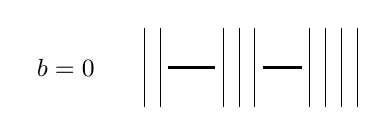
\begin{tikzpicture}
        
      \node at(0, .5)(a){\small{$b=0$}};
      \draw(1, 0) to (1, 1);
      \draw(1.2, 0) to (1.2, 1);
      \draw[line width = .3mm](1.3, .5) to (1.9, .5);
      \draw(2, 0) to (2, 1);
      \draw(2.2, 0) to(2.2, 1);
      \draw(2.4, 0) to (2.4, 1);
      \draw[line width = .3mm](2.5, .5) to (3, .5);
      \draw(3.1, 0) to (3.1, 1);
      \draw(3.3, 0) to (3.3, 1);
      \draw(3.5, 0) to (3.5, 1);
      \draw(3.7, 0) to (3.7, 1);
      \end{tikzpicture}}
  \end{minipage}
   \begin{minipage}{.45\textwidth}
    \centering
      \resizebox{.5\textwidth}{.1\textheight}{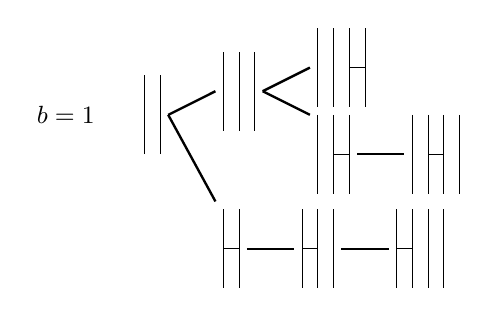
\begin{tikzpicture}
        
      \node at(0, .5)(a){\small{$b=1$}};
        \draw(1, 0) to (1, 1);
        \draw(1.2, 0) to (1.2, 1);
     \draw[line width = .3mm](1.3, .5) to (1.9, .8);
        \draw(2, .3) to (2, 1.3);
        \draw(2.2, .3) to(2.2, 1.3);
        \draw(2.4, .3) to (2.4, 1.3);
      \draw[line width = .3mm](2.5, .8) to (3.1, 1.1);
        \draw(3.2, 0.6) to (3.2, 1.6);
        \draw(3.4, 0.6) to (3.4, 1.6);
        \draw(3.6, 0.6) to (3.6, 1.6);
        \draw(3.6, 1.1) to (3.8, 1.1);
      \draw(3.8, 0.6) to (3.8, 1.6);

     \draw[line width = .3mm](2.5, .8) to (3.1, .5);
        \draw(3.2, .5) to (3.2, -.5);
        \draw(3.4, .5) to (3.4, -.5);
          \draw(3.4, 0) to (3.6, 0);                
        \draw(3.6, .5) to (3.6, -.5);


      \draw[line width = .3mm](3.7, 0) to (4.3, 0);
        \draw(4.4, .5) to (4.4, -.5);
        \draw(4.6, .5) to (4.6, -.5);
        \draw(4.8, .5) to (4.8, -.5);
                  \draw(4.6, 0) to (4.8, 0);                
        \draw(5, .5) to (5, -.5);


        \draw[line width= .3mm](1.3, .5) to (1.9, -.6);
          \draw(2, -.7) to (2, -1.7);
            \draw(2, -1.2) to (2.2, -1.2);
          \draw(2.2, -.7) to (2.2, -1.7);

        \draw[line width= .3mm](2.3, -1.2) to (2.9, -1.2);
        \draw(3, -.7) to (3, -1.7);
            \draw(3, -1.2) to (3.2, -1.2);
        \draw(3.2, -.7) to (3.2, -1.7);
        \draw(3.4, -.7) to (3.4, -1.7);
        \draw[line width= .3mm](3.5, -1.2) to (4.1, -1.2);
        \draw(4.2, -.7) to (4.2, -1.7);
            \draw(4.2, -1.2) to (4.4, -1.2);
        \draw(4.4, -.7) to (4.4, -1.7);
        \draw(4.6, -.7) to (4.6, -1.7);
        \draw(4.8, -.7) to (4.8, -1.7);
        




      \end{tikzpicture}}
      
    \end{minipage}
    \begin{minipage}{.45\textwidth}
      \centering
      \resizebox{.5\textwidth}{.2\textheight}{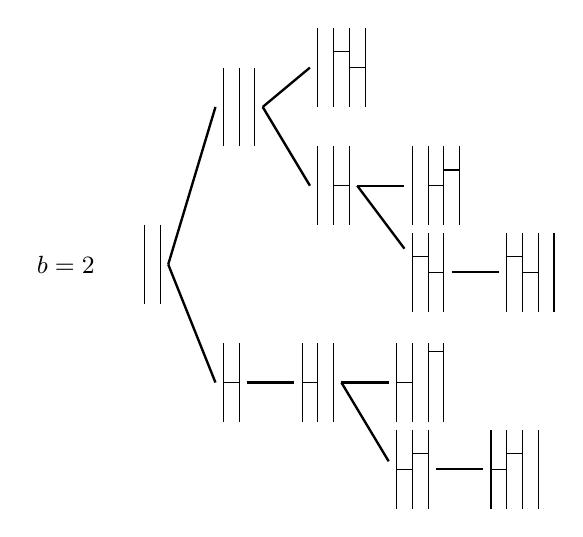
\begin{tikzpicture}
      \node at(0, 5.5){\small{$b=2$}};  
      %%t1
      \draw(1, 5) to (1, 6);
      \draw(1.2, 5) to (1.2, 6);
    \draw[line width = .3mm](1.3, 5.5) to (1.9, 7.5);
      \draw(2, 8) to (2, 7);
      \draw(2.2, 8) to (2.2, 7);
      \draw(2.4, 8) to (2.4, 7);
    \draw[line width = .3mm](2.5, 7.5) to (3.1, 8);
      \draw(3.2, 7.5) to (3.2, 8.5);
      \draw(3.4, 7.5) to (3.4, 8.5);
        \draw(3.4, 8.2) to (3.6, 8.2);
      \draw(3.6, 7.5) to (3.6, 8.5);
        \draw(3.6, 8) to (3.8, 8);
      \draw(3.8, 7.5) to (3.8, 8.5);

      %%tt2
    \draw[line width=.3mm](2.5, 7.5) to (3.1, 6.5);
      \draw(3.2, 7) to (3.2, 6);
      \draw(3.4, 7) to (3.4, 6);
        \draw(3.4, 6.5) to (3.6, 6.5);
      \draw(3.6, 7) to (3.6, 6);
    
    \draw[line width = .3mm](3.7, 6.5) to (4.3, 6.5);
      \draw(4.4, 6) to (4.4, 7);
      \draw(4.6, 6) to (4.6, 7);
        \draw(4.6, 6.5) to (4.8, 6.5);
      \draw(4.8, 6) to (4.8, 7);
        \draw(4.8, 6.7) to (5, 6.7);
      \draw(5, 6) to (5, 7);
    
    \draw[line width = .3mm](3.7, 6.5) to (4.3, 5.7);
      \draw(4.4, 5.9) to (4.4, 4.9);
        \draw(4.4, 5.6) to (4.6, 5.6);
      \draw(4.6, 5.9) to (4.6, 4.9);
        \draw(4.6, 5.4) to (4.8, 5.4);
      \draw(4.8, 5.9) to (4.8, 4.9);
    
   \draw[line width = .3mm](4.9, 5.4) to (5.5, 5.4);
      \draw(5.6, 5.9) to (5.6, 4.9);
        \draw(5.6, 5.6) to (5.8, 5.6);
      \draw(5.8, 5.9) to (5.8, 4.9);
        \draw(5.8, 5.4) to (6, 5.4);
      \draw(6, 5.9) to (6, 4.9);
      \draw(6.2, 5.9) to (6.2, 4.9);

    \draw[line width = .3mm](1.3, 5.5) to (1.9, 4);
    
        \draw(2, 4.5) to (2, 3.5);
          \draw(2, 4) to (2.2, 4);
        \draw(2.2, 4.5) to (2.2, 3.5);

    \draw[line width = .3mm](2.3, 4) to (2.9, 4);
        \draw(3, 4.5) to (3, 3.5);
          \draw(3, 4) to (3.2, 4);
        \draw(3.2, 4.5) to (3.2, 3.5);
        \draw(3.4, 4.5) to (3.4, 3.5);
    \draw[line width = .3mm](3.5, 4) to (4.1, 4);
    \draw[line width = .3mm](3.5, 4) to (4.1, 3);
      \draw(4.2, 4.5) to (4.2, 3.5);
        \draw(4.2, 4) to (4.4, 4);
      \draw(4.4, 4.5) to (4.4, 3.5);
      \draw(4.6, 4.5) to (4.6, 3.5);
        \draw(4.6, 4.4) to (4.8, 4.4);
      \draw(4.8, 4.5) to (4.8, 3.5);

      \draw(4.2, 3.4) to (4.2, 2.4);
        \draw(4.2, 2.9) to (4.4, 2.9);
      \draw(4.4, 3.4) to (4.4, 2.4);
        \draw(4.4, 3.1) to (4.6, 3.1);
      \draw(4.6, 3.4) to (4.6, 2.4);
    
    \draw[line width = .3mm](4.7, 2.9) to (5.3, 2.9);
        \draw(5.4, 3.4) to (5.4, 2.4);
          \draw(5.4, 2.9) to (5.6, 2.9);
        \draw(5.6, 3.4) to (5.6, 2.4);
          \draw(5.6, 3.1) to (5.8, 3.1);
        \draw(5.8, 3.4) to (5.8, 2.4);
        \draw(6.0, 3.4) to (6.0, 2.4);




    \end{tikzpicture}}
  \end{minipage}
  \begin{minipage}{.45\textwidth}
    \centering
    \resizebox{.5\textwidth}{.25\textheight}{\begin{tikzpicture}
      \node at(0, 5.5){\small{$b=3$}};
        %%t1
        \draw(1, 5) to (1, 6);
        \draw(1.2, 5) to (1.2, 6);
      \draw[line width = .3mm](1.3, 5.5) to (1.9, 7.5);
        \draw(2, 7) to (2, 8);
        \draw(2.2, 7) to (2.2, 8);
        \draw(2.4, 7) to (2.4, 8);
      \draw[line width = .3mm](2.5, 7.5) to (2.9, 9);
      \draw[line width = .3mm](2.5, 7.5) to (2.9, 6.5);
        %%Leaf1
        \draw(3, 9.5) to (3, 8.5);
          \draw(3, 9.4) to (3.2, 9.4);
        \draw(3.2, 9.5) to (3.2, 8.5);
          \draw(3.2, 9.2) to (3.4, 9.2);
        \draw(3.4, 9.5) to (3.4, 8.5);
          \draw(3.4, 9) to (3.6, 9);
        \draw(3.6, 9.5) to (3.6, 8.5);
        %%t2
        \draw(3, 7) to (3, 6);
        \draw(3.2, 7) to (3.2, 6);
          \draw(3.2, 6.5) to (3.4, 6.5);
        \draw(3.4, 7) to (3.4, 6);
        \draw[line width = .3mm](3.5, 6.5) to (4.1, 6.5);
        \draw[line width = .3mm](3.5, 6.5) to (4.1, 5.5);
        %%Leaf2
        \draw(4.2, 6) to (4.2, 7);
        \draw(4.4, 6) to (4.4, 7);
          \draw(4.4, 6.7) to (4.6, 6.7);
          \draw(4.4, 6.3) to (4.6, 6.3);
        \draw(4.6, 6) to (4.6, 7);
          \draw(4.6, 6.5) to (4.8, 6.5);
        \draw(4.8, 6) to (4.8, 7);

        \draw(4.2, 5.9) to (4.2, 4.9);
          \draw(4.2, 5.5) to (4.4, 5.5);
        \draw(4.4, 5.9) to (4.4, 4.9);
          \draw(4.4, 5.3) to (4.6, 5.3);
        \draw(4.6, 5.9) to (4.6, 4.9);
      \draw[line width = .3mm](4.7, 5.4) to (5.3, 5.4);
      %%leaf 3
        \draw(5.4, 4.9) to (5.4, 5.9);
          \draw(5.4, 5.5)to(5.6, 5.5);
        \draw(5.6, 4.9) to (5.6, 5.9);
          \draw(5.6, 5.3) to (5.8, 5.3);
        \draw(5.8, 4.9) to (5.8, 5.9);
          \draw(5.8, 5.5)to(6, 5.5);
        \draw(6.0, 4.9) to (6.0, 5.9);

      %%Line
      \draw[line width=.3mm](1.3, 5.5) to (1.9, 4);

        \draw(2, 4.5) to (2, 3.5);
          \draw(2, 3.6) to (2.2, 3.6);
        \draw(2.2, 4.5) to (2.2, 3.5);

      \draw[line width = .3mm](2.3, 4) to (2.9, 4);
        \draw(3.0, 4.5) to (3.0, 3.5);
          \draw(3, 3.6) to (3.2, 3.6);
        \draw(3.2, 4.5) to (3.2, 3.5);
      
        \draw(3.4, 4.5) to (3.4, 3.5);
      
        \draw[line width = .3mm](3.5, 4) to (4.1, 4.3);
      %%leaf 4
        \draw(4.2, 3.8) to (4.2, 4.8);
          \draw(4.2, 3.9) to (4.4, 3.9);
        \draw(4.4, 3.8) to (4.4, 4.8);
          \draw(4.4, 4.5) to (4.6, 4.5);
        \draw(4.6, 3.8) to (4.6, 4.8);
          \draw(4.6, 4.3) to (4.8, 4.3);
        \draw(4.8, 3.8) to (4.8, 4.8);

    \draw[line width = .3mm](3.5, 4) to (4.1, 3.5);
      \draw(4.2, 3.7) to (4.2, 2.7);
        \draw(4.2,  2.8) to (4.4, 2.8);
      \draw(4.4, 3.7) to (4.4, 2.7);
        \draw(4.4, 3) to (4.6, 3);
      \draw(4.6, 3.7) to (4.6, 2.7);

    \draw[line width = .3mm](4.7, 3.2) to (5.3, 3.9);
    %%leaf 5
      \draw(5.4, 4.4) to (5.4, 3.4);
        \draw(5.4, 3.5) to (5.6, 3.5);
        \draw(5.6, 3.7) to (5.8, 3.7);
        \draw(5.8, 3.9) to (6.0, 3.9);
      \draw(5.6, 4.4) to (5.6, 3.4);
      \draw(5.8, 4.4) to (5.8, 3.4);
      \draw(6.0, 4.4) to (6.0, 3.4);
   
    \draw[line width = .3mm](4.7, 3.2) to (5.3, 2.5);
    \draw(5.4, 3) to (5.4, 2);
      \draw(5.4, 2.1) to (5.6, 2.1);
      \draw(5.4, 2.5) to (5.6, 2.5);
    \draw(5.6, 3) to (5.6, 2);
      \draw(5.6, 2.3) to (5.8, 2.3);
    \draw(5.8, 3) to (5.8, 2);

    \draw[line width = .3mm](5.9, 2.5) to (6.4, 2.5);
    \draw(6.5, 3) to (6.5, 2);
      \draw(6.5, 2.1) to (6.7, 2.1);
      \draw(6.5, 2.5) to (6.7, 2.5);
    \draw(6.7, 3) to (6.7, 2);
      \draw(6.7, 2.3) to (6.9, 2.3);
    \draw(6.9, 3) to (6.9, 2);
    \draw(7.1, 3) to (7.1, 2);




    \end{tikzpicture}}
  \end{minipage}
   \begin{minipage}{.45\textwidth}
    \centering
    \resizebox{.5\textwidth}{.25\textheight}{\begin{tikzpicture}
      \node at(0, 5.5){\small{$b=4$}};
        %%t1
        \draw(1, 5) to (1, 6);
        \draw(1.2, 5) to (1.2, 6);
      \draw[line width = .3mm](1.3, 5.5) to (1.9, 7.5);
        \draw(2, 7) to (2, 8);
        \draw(2.2, 7) to (2.2, 8);
        \draw(2.4, 7) to (2.4, 8);
      \draw[line width = .3mm](2.5, 7.5) to (2.9, 9);
      \draw[line width = .3mm](2.5, 7.5) to (2.9, 7.5);
        %%Leaf1
        \draw(3, 9.5) to (3, 8.5);
          \draw(3, 9.4) to (3.2, 9.4);
        \draw(3.2, 9.5) to (3.2, 8.5);
          \draw(3.2, 9.2) to (3.4, 9.2);
        \draw(3.4, 9.5) to (3.4, 8.5);
          \draw(3.4, 9) to (3.6, 9);
        \draw(3.6, 9.5) to (3.6, 8.5);
        %%t2
        \draw(3, 7) to (3, 8);
        \draw(3.2, 7) to (3.2, 8);
          \draw(3.2, 7.5) to (3.4, 7.5);
        \draw(3.4, 7) to (3.4, 8);
        \draw[line width = .3mm](3.5, 7.5) to (4.1, 7.5);
        %%Leaf2
        \draw(4.2, 7) to (4.2, 8);
          \draw(4.2, 7.9) to (4.4, 7.9);
        \draw(4.4, 7) to (4.4, 8);
          \draw(4.4, 7.3) to (4.6, 7.3);
          \draw(4.4, 7.7) to (4.6, 7.7);
        \draw(4.6, 7) to (4.6, 8);
          \draw(4.6, 7.5) to (4.8, 7.5);s
        \draw(4.8, 7) to (4.8, 8);
        %%\draw[line width = .3mm](3.5, 6.5) to (4.1, 5.5);

        \draw[line width = .3mm](3.5, 7.5) to (4.1, 6.5);

        \draw(4.2, 6.9) to (4.2, 5.9);
          \draw(4.2, 6.4) to (4.4, 6.4);
        \draw(4.4, 6.9) to (4.4, 5.9);
          \draw(4.4, 6.2) to (4.6, 6.2);
        \draw(4.6, 6.9) to (4.6, 5.9);

        \draw[line width = .3mm](4.7, 6.4) to (5.3, 6.4);
      %%leaf 3
        \draw(5.4, 6.9) to (5.4, 5.9);
          \draw(5.4, 6.4) to (5.6, 6.4);
        \draw(5.6, 6.9) to (5.6, 5.9);
          \draw(5.6, 6.2) to (5.8, 6.2);
          \draw(5.6, 6.6) to (5.8, 6.6);
        \draw(5.8, 6.9) to (5.8, 5.9);
          \draw(5.8, 6.4) to (6.0, 6.4);
        \draw(6.0, 6.9) to (6.0, 5.9);


      \draw[line width = .3mm](1.3, 5.5) to (1.9, 3.5);
      \draw(1.9, 4) to (1.9, 3);
        \draw(1.9, 3.1) to (2.1, 3.1);
      \draw(2.1, 4) to (2.1, 3);

      \draw[line width = .3mm](2.2, 3.5) to (2.8, 4.1);
      
      \draw(2.9, 4.6) to (2.9, 3.6);
        \draw(2.9, 3.7) to (3.1, 3.7);
      \draw(3.1, 4.6) to (3.1, 3.6);
      \draw(3.3, 4.6) to (3.3, 3.6);

      \draw[line width = .3mm](3.4, 4.1) to (4,5.1);
      %%Leaf 4
      \draw(4.1, 5.6) to (4.1, 4.6);
        \draw(4.1, 4.7) to (4.3, 4.7);
        \draw(4.1, 5.5) to (4.3, 5.5);
      \draw(4.3, 4.6) to (4.3, 5.6);
        \draw(4.3, 5.3) to (4.5, 5.3);
      \draw(4.5, 4.6) to (4.5, 5.6);
        \draw(4.5, 5.1) to (4.7, 5.1);
      \draw(4.7, 4.6) to (4.7, 5.6);

      \draw[line width = .3mm](3.4, 4.1) to (4,3.1);
      \draw(4.1, 3.6) to (4.1, 2.6);
        \draw(4.1, 2.7) to (4.3, 2.7);
      \draw(4.3, 3.6) to (4.3, 2.6);
        \draw(4.3, 2.9) to (4.5, 2.9);
      \draw(4.5, 3.6) to (4.5, 2.6);

      \draw[line width = .3mm](4.6, 3.1) to (5.2, 3.8);
      %%leaf 5
      \draw(5.3, 4.3) to (5.3, 3.3);
        \draw(5.3, 3.4) to (5.5, 3.4);
      \draw(5.5, 4.3) to (5.5, 3.3);
        \draw(5.5, 3.6) to (5.7, 3.6);
      \draw(5.7, 4.3) to (5.7, 3.3);
        \draw(5.7, 3.8) to (5.9, 3.8);
        \draw(5.5, 4) to (5.7, 4);
      \draw(5.9, 4.3) to (5.9, 3.3);
      
      
      \draw[line width = .3mm](4.6, 3.1) to (5.2, 2.5);

      \draw(5.3, 3) to (5.3, 2);
        \draw(5.3, 2.1) to (5.5, 2.1);
        \draw(5.3, 2.5) to (5.5, 2.5);
      \draw(5.5, 3) to (5.5, 2);
        \draw(5.5, 2.3) to (5.7, 2.3);
      \draw(5.7, 3) to (5.7, 2);

      \draw[line width = .3mm](5.8, 2.5) to (6.4, 2.5);

      
      \draw(6.5, 3) to (6.5, 2);
        \draw(6.5, 2.1) to (6.7, 2.1);
        \draw(6.5, 2.5) to (6.7, 2.5);
      \draw(6.7, 3) to (6.7, 2);
        \draw(6.7, 2.3) to (6.9, 2.3);
      \draw(6.9, 3) to (6.9, 2);
        \draw(6.9, 2.5) to (7.1, 2.5);
      \draw(7.1, 2) to (7.1, 3);






    \end{tikzpicture}}
  \end{minipage}
  \begin{minipage}{.45\textwidth}
    \centering
    \resizebox{.5\textwidth}{.25\textheight}{\begin{tikzpicture}
      \node at(0, 5.5){\small{$b=5$}};
        %%t1
        \draw(1, 5) to (1, 6);
        \draw(1.2, 5) to (1.2, 6);
      \draw[line width = .3mm](1.3, 5.5) to (1.9, 7.5);
        \draw(2, 7) to (2, 8);
        \draw(2.2, 7) to (2.2, 8);
        \draw(2.4, 7) to (2.4, 8);
      \draw[line width = .3mm](2.5, 7.5) to (2.9, 9);
      \draw[line width = .3mm](2.5, 7.5) to (2.9, 7.5);
        %%Leaf1
        \draw(3, 9.5) to (3, 8.5);
          \draw(3, 9.4) to (3.2, 9.4);
        \draw(3.2, 9.5) to (3.2, 8.5);
          \draw(3.2, 9.2) to (3.4, 9.2);
        \draw(3.4, 9.5) to (3.4, 8.5);
          \draw(3.4, 9) to (3.6, 9);
        \draw(3.6, 9.5) to (3.6, 8.5);
        %%t2
        \draw(3, 7) to (3, 8);
        \draw(3.2, 7) to (3.2, 8);
          \draw(3.2, 7.5) to (3.4, 7.5);
        \draw(3.4, 7) to (3.4, 8);
        \draw[line width = .3mm](3.5, 7.5) to (4.1, 7.5);
        %%Leaf2
        \draw(4.2, 7) to (4.2, 8);
          \draw(4.2, 7.9) to (4.4, 7.9);
        \draw(4.4, 7) to (4.4, 8);
          \draw(4.4, 7.3) to (4.6, 7.3);
          \draw(4.4, 7.7) to (4.6, 7.7);
        \draw(4.6, 7) to (4.6, 8);
          \draw(4.6, 7.5) to (4.8, 7.5);
        \draw(4.8, 7) to (4.8, 8);
        \draw[line width = .3mm](3.5, 7.5) to (4.1, 6.5);

        \draw[line width = .3mm](3.5, 7.5) to (4.1, 6.5);

        \draw(4.2, 6.9) to (4.2, 5.9);
          \draw(4.2, 6.4) to (4.4, 6.4);
        \draw(4.4, 6.9) to (4.4, 5.9);
          \draw(4.4, 6.2) to (4.6, 6.2);
        \draw(4.6, 6.9) to (4.6, 5.9);

        \draw[line width = .3mm](4.7, 6.4) to (5.3, 6.4);
      %%leaf 3
        \draw(5.4, 6.9) to (5.4, 5.9);
          \draw(5.4, 6.4) to (5.6, 6.4);
          \draw(5.4, 6.8) to (5.6, 6.8);
        \draw(5.6, 6.9) to (5.6, 5.9);
          \draw(5.6, 6.2) to (5.8, 6.2);
          \draw(5.6, 6.6) to (5.8, 6.6);
        \draw(5.8, 6.9) to (5.8, 5.9);
          \draw(5.8, 6.4) to (6.0, 6.4);
        \draw(6.0, 6.9) to (6.0, 5.9);


      \draw[line width = .3mm](1.3, 5.5) to (1.9, 3.5);
      \draw(1.9, 4) to (1.9, 3);
        \draw(1.9, 3.1) to (2.1, 3.1);
      \draw(2.1, 4) to (2.1, 3);

      \draw[line width = .3mm](2.2, 3.5) to (2.8, 4.1);
      
      \draw(2.9, 4.6) to (2.9, 3.6);
        \draw(2.9, 3.7) to (3.1, 3.7);
      \draw(3.1, 4.6) to (3.1, 3.6);
      \draw(3.3, 4.6) to (3.3, 3.6);

      \draw[line width = .3mm](3.4, 4.1) to (4,5.1);
      %%Leaf 4
      \draw(4.1, 5.6) to (4.1, 4.6);
        \draw(4.1, 4.7) to (4.3, 4.7);
        \draw(4.1, 5.5) to (4.3, 5.5);
      \draw(4.3, 4.6) to (4.3, 5.6);
        \draw(4.3, 5.3) to (4.5, 5.3);
      \draw(4.5, 4.6) to (4.5, 5.6);
        \draw(4.5, 5.1) to (4.7, 5.1);
      \draw(4.7, 4.6) to (4.7, 5.6);

      \draw[line width = .3mm](3.4, 4.1) to (4,3.1);
      \draw(4.1, 3.6) to (4.1, 2.6);
        \draw(4.1, 2.7) to (4.3, 2.7);
      \draw(4.3, 3.6) to (4.3, 2.6);
        \draw(4.3, 2.9) to (4.5, 2.9);
      \draw(4.5, 3.6) to (4.5, 2.6);

      \draw[line width = .3mm](4.6, 3.1) to (5.2, 3.8);
      %%leaf 5
      \draw(5.3, 4.3) to (5.3, 3.3);
        \draw(5.3, 3.4) to (5.5, 3.4);
        \draw(5.3, 4.2) to (5.5, 4.2);

      \draw(5.5, 4.3) to (5.5, 3.3);
        \draw(5.5, 3.6) to (5.7, 3.6);
      \draw(5.7, 4.3) to (5.7, 3.3);
        \draw(5.7, 3.8) to (5.9, 3.8);
        \draw(5.5, 4) to (5.7, 4);
      \draw(5.9, 4.3) to (5.9, 3.3);
      
      
      \draw[line width = .3mm](4.6, 3.1) to (5.2, 2.5);

      \draw(5.3, 3) to (5.3, 2);
        \draw(5.3, 2.1) to (5.5, 2.1);
        \draw(5.3, 2.5) to (5.5, 2.5);
      \draw(5.5, 3) to (5.5, 2);
        \draw(5.5, 2.3) to (5.7, 2.3);
      \draw(5.7, 3) to (5.7, 2);

      \draw[line width = .3mm](5.8, 2.5) to (6.4, 2.5);

      
      \draw(6.5, 3) to (6.5, 2);
        \draw(6.5, 2.1) to (6.7, 2.1);
        \draw(6.5, 2.5) to (6.7, 2.5);
      \draw(6.7, 3) to (6.7, 2);
        \draw(6.7, 2.3) to (6.9, 2.3);
      \draw(6.9, 3) to (6.9, 2);
        \draw(6.9, 2.5) to (7.1, 2.5);
      \draw(7.1, 2) to (7.1, 3);






    \end{tikzpicture}}
  \end{minipage}
  
  

     
  \caption{The forest for all ladders in $CanL\{\pi_{4}\}$ generated by the Cyclic Inversion Algorithm. The first tree has all ladders with zero bars, the second tree 
  has all ladders with 1 bar, etc.}
  \label{Fig:CanLForest}
\end{figure}
\end{center}\pagebreak




It has been stated that the forest created by the Cyclic Inversion algorithm generates $CanL\{\pi_{N}\}$. This claim has 
yet to have been proven, so the following theorem will prove this claim.

\begin{theorem}
  
  The forest created by the Cyclic Inversion algorithm generates $CanL\{\pi_{N}\}$
\end{theorem}
\begin{proof}
  The proof is done by way of a combinatorial proof and induction. Rather than list ladders, we shall list permutations using the same method.  
  Let $List(N, K)$ be the listing of permutations of order $N$ with $K$ inversions. The hypothesis is that $List(N, K)=\sum_{M=0}^{K} List(N-1, M)$ 
  given $N>1$ and $K \geq 0$.
  The base case is $N=2$ and $K=0$. We know that the identity permutation of order $1$ has no inversions. We know that the list containing the identity 
  permutation of order $1$ is of length one. We know that the list containing the identity permutation of order $2$ is of length one. By appending the 
  value $2$ to the only permutation in the list $List(1, 0)$ we get the only permutation in the list $List(2, 0)$. Therefore the base case checks out.
  
  Suppose we have the list of permutations for $List(N-1, 0) \dots List(N-1, K)$. We want to show that we can insert the $Nth$ element into each of the
  permutations in each of these lists such that the resulting permutations have $N$ elements with $K$ inversions. Partition $K$ into $K'$ and $K''$. Note that 
  $K'+K''=K$.
  Let $K'$ equal the number of inversions formed by the $Nth$ element. Let $K''$ equal the number of elements not formed by the $Nth$ element.
  We can look at the $List(N-1, 0) \dots List(N-1, K)$ as lists of permutations with $K''$ inversions. So we write 
  $List(N-1, 0) \dots List(N-1, K)$ as $List(N-1, K''=0) \dots List(N-1, K''=K)$. When $K''=0$ we know $List(N-1, 0)$ has one permutation, thus $K'=K$.
  The $Nth$ element must be positioned $K'$ positions to the left of the $Nth$ position in this one permutation from $List(N-1, 0)$ to form a permutation of order $N$ with $K$ inversions. 
  In general, we can say that for each of the permutations from each of the $List(N-1, K'')$, we know that the $Nth$ element must be postioned $K-K''$ to the left of the $Nth$ position in order to 
  create a permutation of length $N$ with $K$ inversions. Thus, by exhaustively inserting the $Nth$ element in all $K-K''=K'$ positions to the left of the $Nth$ position 
  in all permutations from all $List(N-1, K'')$, we get all permutations of order $N$ with $K$ inversions. 
  Therefore $List(N, K) = List(N, K') + \sum_{K''=0}^{K} List(N-1, K'') $.
  Seeing as an inversion in a permutation corresponds to a bar in 
  a ladder, then by using this same proof on ladders, we can generate all ladders with $K$ bars. 
  Which is to say that $Ladders(N, K) = Ladders(N, K') + \sum_{K''=0}^{K} Ladders(N-1, K'')$.
  In order to list $CanL\{\pi_{N}\}$ simply apply this same logic for all $K$ bars for $0 \leq K \leq N(N-1)/2$. To see an example of the above proof for $List(4, 2)$ refer to Table \ref{Table:List4,2}.

\end{proof}

\begin{table}
  \begin{tabular}{|p{2cm}||p{2cm}||p{2cm}||p{2cm} ||p{2cm} ||p{2cm}||}
     \hline
        \small{$N$ value}& \small{$K$ value} & \small{$K''$ value} & \small{$K'$ value} &\small{$L($N-1$, K'')$} & \small{$L(N, K)$}\\
        \hline
        \small{$4$} & \small{$2$} & \small{$0$} & \small{$2$} & \small{$(1,2,3)$} & \small{$(1,4,2,3)$} \\
        \hline
        \small{$4$} & \small{$2$} & \small{$1$} & \small{$1$} & \small{$(1,3,2)$} & \small{$(1,3,4,2)$} \\
        \small{$4$} & \small{$2$} & \small{$1$} & \small{$1$} & \small{$(2,1,3)$} & \small{$(2,1,4,3)$} \\
        \hline
        \small{$4$} & \small{$2$} & \small{$2$} & \small{$0$} & \small{$(3,1,2)$} & \small{$(3,1,2,4)$} \\                
        \small{$4$} & \small{$2$} & \small{$2$} & \small{$0$} & \small{$(2,3,1)$} & \small{$(2,3,1,4)$} \\
        \hline
  \end{tabular}
  \caption{The table showing all $List(4, 2)$ derived from $List(3, 0) \dots List(3, 2) + List(4, K')$}
  \label{Table:List4,2}
\end{table}




